\documentclass{article}
\usepackage{graphicx} % Required for inserting images
\usepackage{subcaption}
\usepackage{booktabs}
\usepackage{tabularx}
\usepackage{verbatim}
\usepackage{pythonhighlight}

\title{Exploring Language Patterns in NIPS Papers using K-Means Clustering}
\author{Lorenzo Mendoza}
\date{April 2023}

\begin{document}

\maketitle

\section{Introduction}
In this assignment we are asked to carry out a clustering routing using the K-means clustering methods and analyzed the outputs. We will be using the scikit-learn \cite{scikit-learn-clustering} module for our algorithm implementation along with plotly \cite{Plotly} and matplotlib \cite{Matplotlib} for the visuals.

\section{Data Preprocessing}
We use the NIPS dataset from the Bag of Words data \cite{Dua2019} in the UCI database for this assignment. NIPS stands for Neural Information Processing Systems. It is an annual conference that brings together researchers from a variety of fields, including machine learning, artificial intelligence, computational neuroscience, and cognitive science. The conference features presentations of new research findings, workshops, tutorials, and other events aimed at fostering collaboration and the exchange of ideas among researchers. The data has already been cleaned and vectorized so we can skip the text preprocessing and vectorization process. However, we carry out stardarization using the ‘StandardScalar‘ class in scikit-learn.



\section{KMeans Algorithm}
\subsection{KMeans Algorithm}
The KMeans algorithm partitions N data points into K clusters C through an iterative process based on centroids \cite{satishgunjal-kmeans-tutorial}. The assignment of each data point $x_i$ to a cluster is determined by minimizing its Euclidean distance from the cluster center $\mu_j$.
\begin{equation}
\min_{C} \sum_{i=1}^{n} \min_{\mu_j \in C} ||x_i - \mu_j||^2
\end{equation}

In scikit-learn's implementation, KMeans++ is used to initialize the centroids by utilizing all data points instead of random initialization. The key parameter in KMeans is the number of clusters K, which we can determine using the elbow method to find the optimal value of K.

\begin{figure}[h]
    \centering
    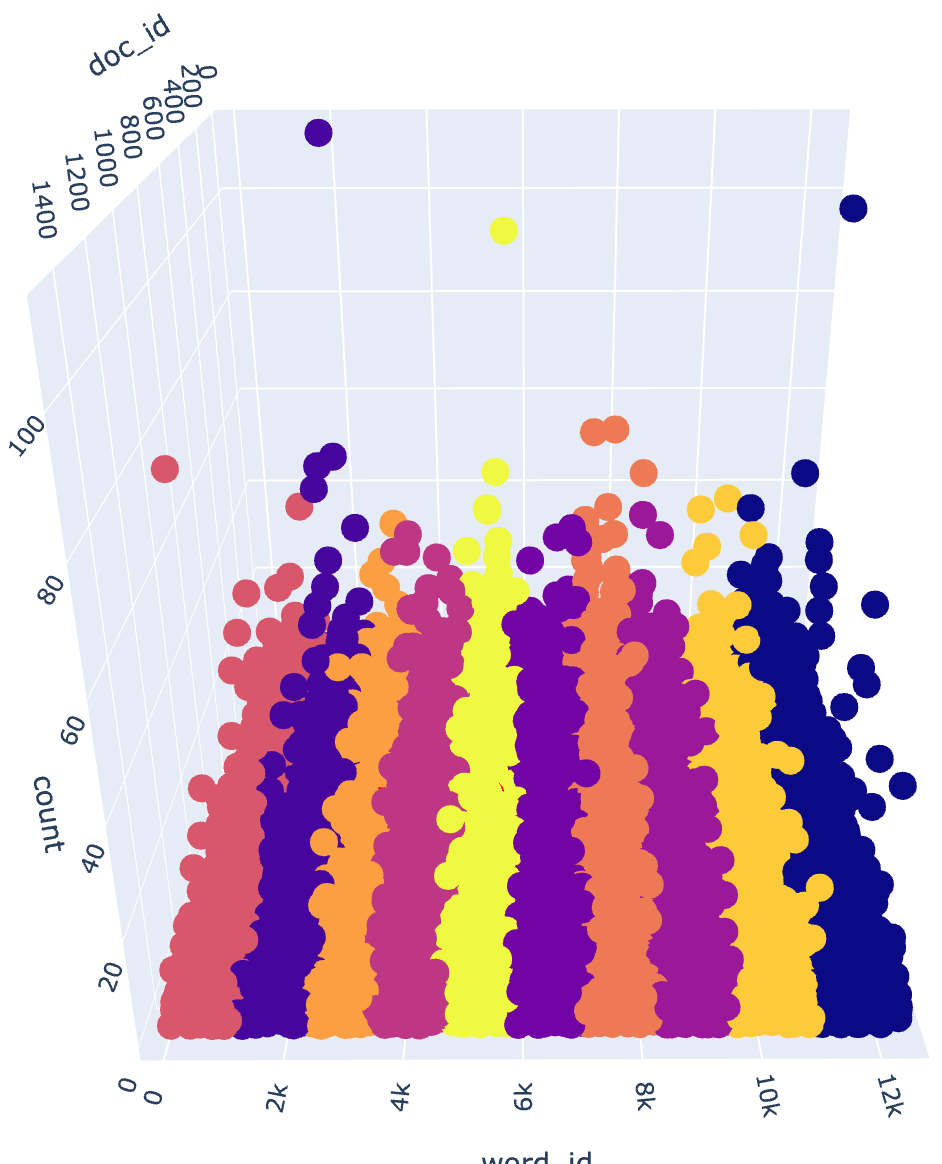
\includegraphics[width=.5\textwidth]{figs/k10.png}
    \caption{3 Dimensional plot with labeled clusters at k=10. Dimensions are $word\_id$, $doc\_id$, and $count$.}
\end{figure}

\subsection{Elbow Method}
The elbow method is a popular technique for finding the optimal value of K in KMeans clustering\cite{satishgunjal-kmeans-tutorial}. It involves plotting the values of the cost function (also known as inertia) against different values of K and looking for the "elbow" point, where the cost function starts to decrease at a slower rate. The optimal value of K is usually the value at which the cost function starts to plateau or the slope of the curve flattens out.

To apply the elbow method, we first fit the KMeans algorithm to our data for different values of K. In our case, we chose to vary K from 1 to 10. For each value of K, we computed the value of the cost function using the "inertia" attribute of the KMeans object. We then plotted these values against the corresponding values of K.



\begin{figure}[h]
    \centering
    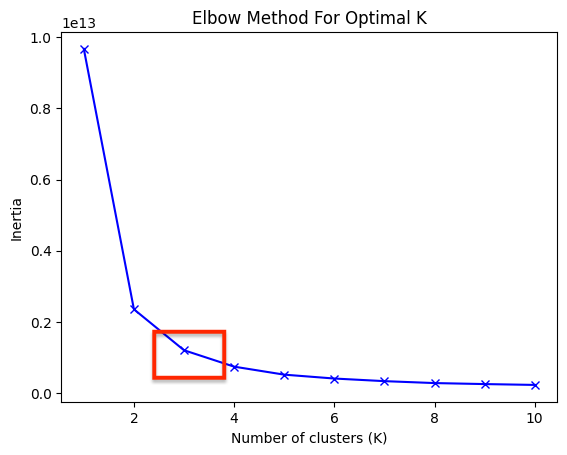
\includegraphics[width=.4\textwidth]{figs/elbow.png}
    \caption{Elbow method performed on dataset from range of 1-10 showing an optimal value of k=3}
\end{figure}

In our implementation, we used the "matplotlib" library to plot the elbow curve. Figure 2 shows the resulting plot. As we can see from the plot, the curve starts to flatten out at around K=3, suggesting that this is the optimal value of K for our data.


\section{Output}


\subsection{3 Dimensions}

In order to perform clustering analysis on the dataset, K-means clustering algorithm was used with k=3. The results were plotted using Plotly to create 3D scatter plots. This analysis was conducted to explore the relationship between the variables and gain insights into the underlying structure of the dataset.
\begin{figure}[h]
    \centering
    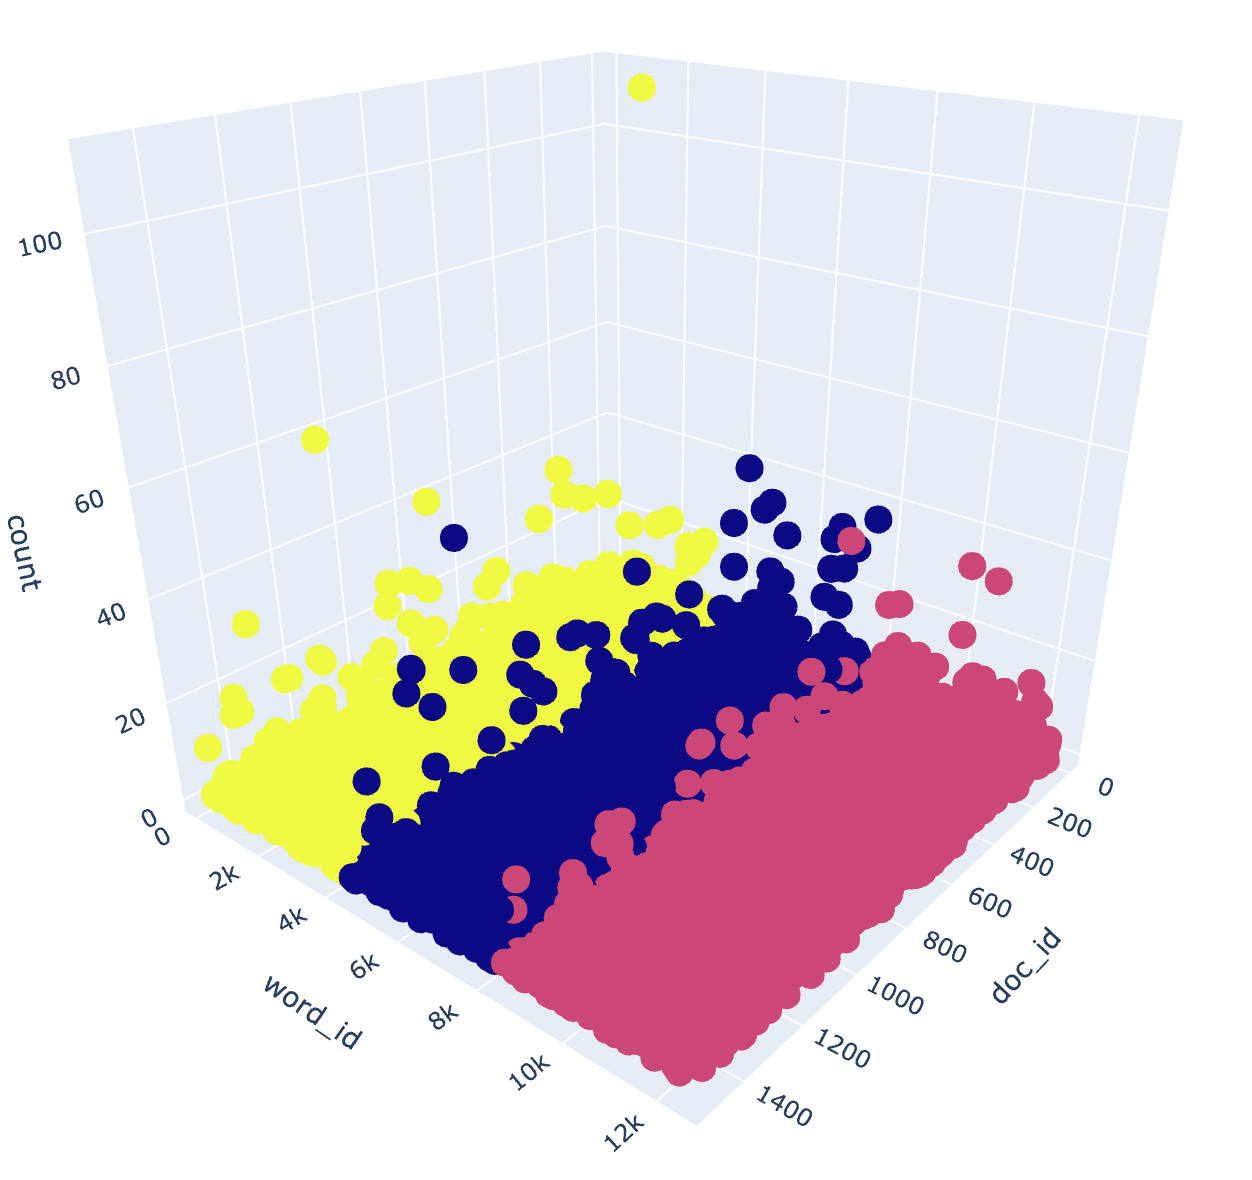
\includegraphics[width=.4\textwidth]{figs/3d.png}
    \caption{3 Dimensional plot with optimal number of clusters determined by elbow method k = 3. Dimensions are $word\_id$, $doc\_id$, and $count$.}
\end{figure}

The 3D scatter plots revealed interesting patterns in the data. Each point in the plot represents a document in the dataset, with its location determined by its values on three variables: $doc\_id$, $word\_id$, and count. The three clusters identified by the K-means algorithm were clearly visible in the plots.

However, the plots also revealed some intriguing patterns that needed to be examined more closely. To further investigate these patterns, 2D scatter plots were created for the $doc\_id-word\_id$, $count-word\_id$, and $count-doc\_id$ axes. These plots allowed for a closer examination of the relationships between these variables and revealed more details about the structure of the data. The insights gained from these plots were used to refine the analysis and gain a deeper understanding of the dataset.


\subsection{Axis to Axis}

\begin{figure}[h]
    \centering
    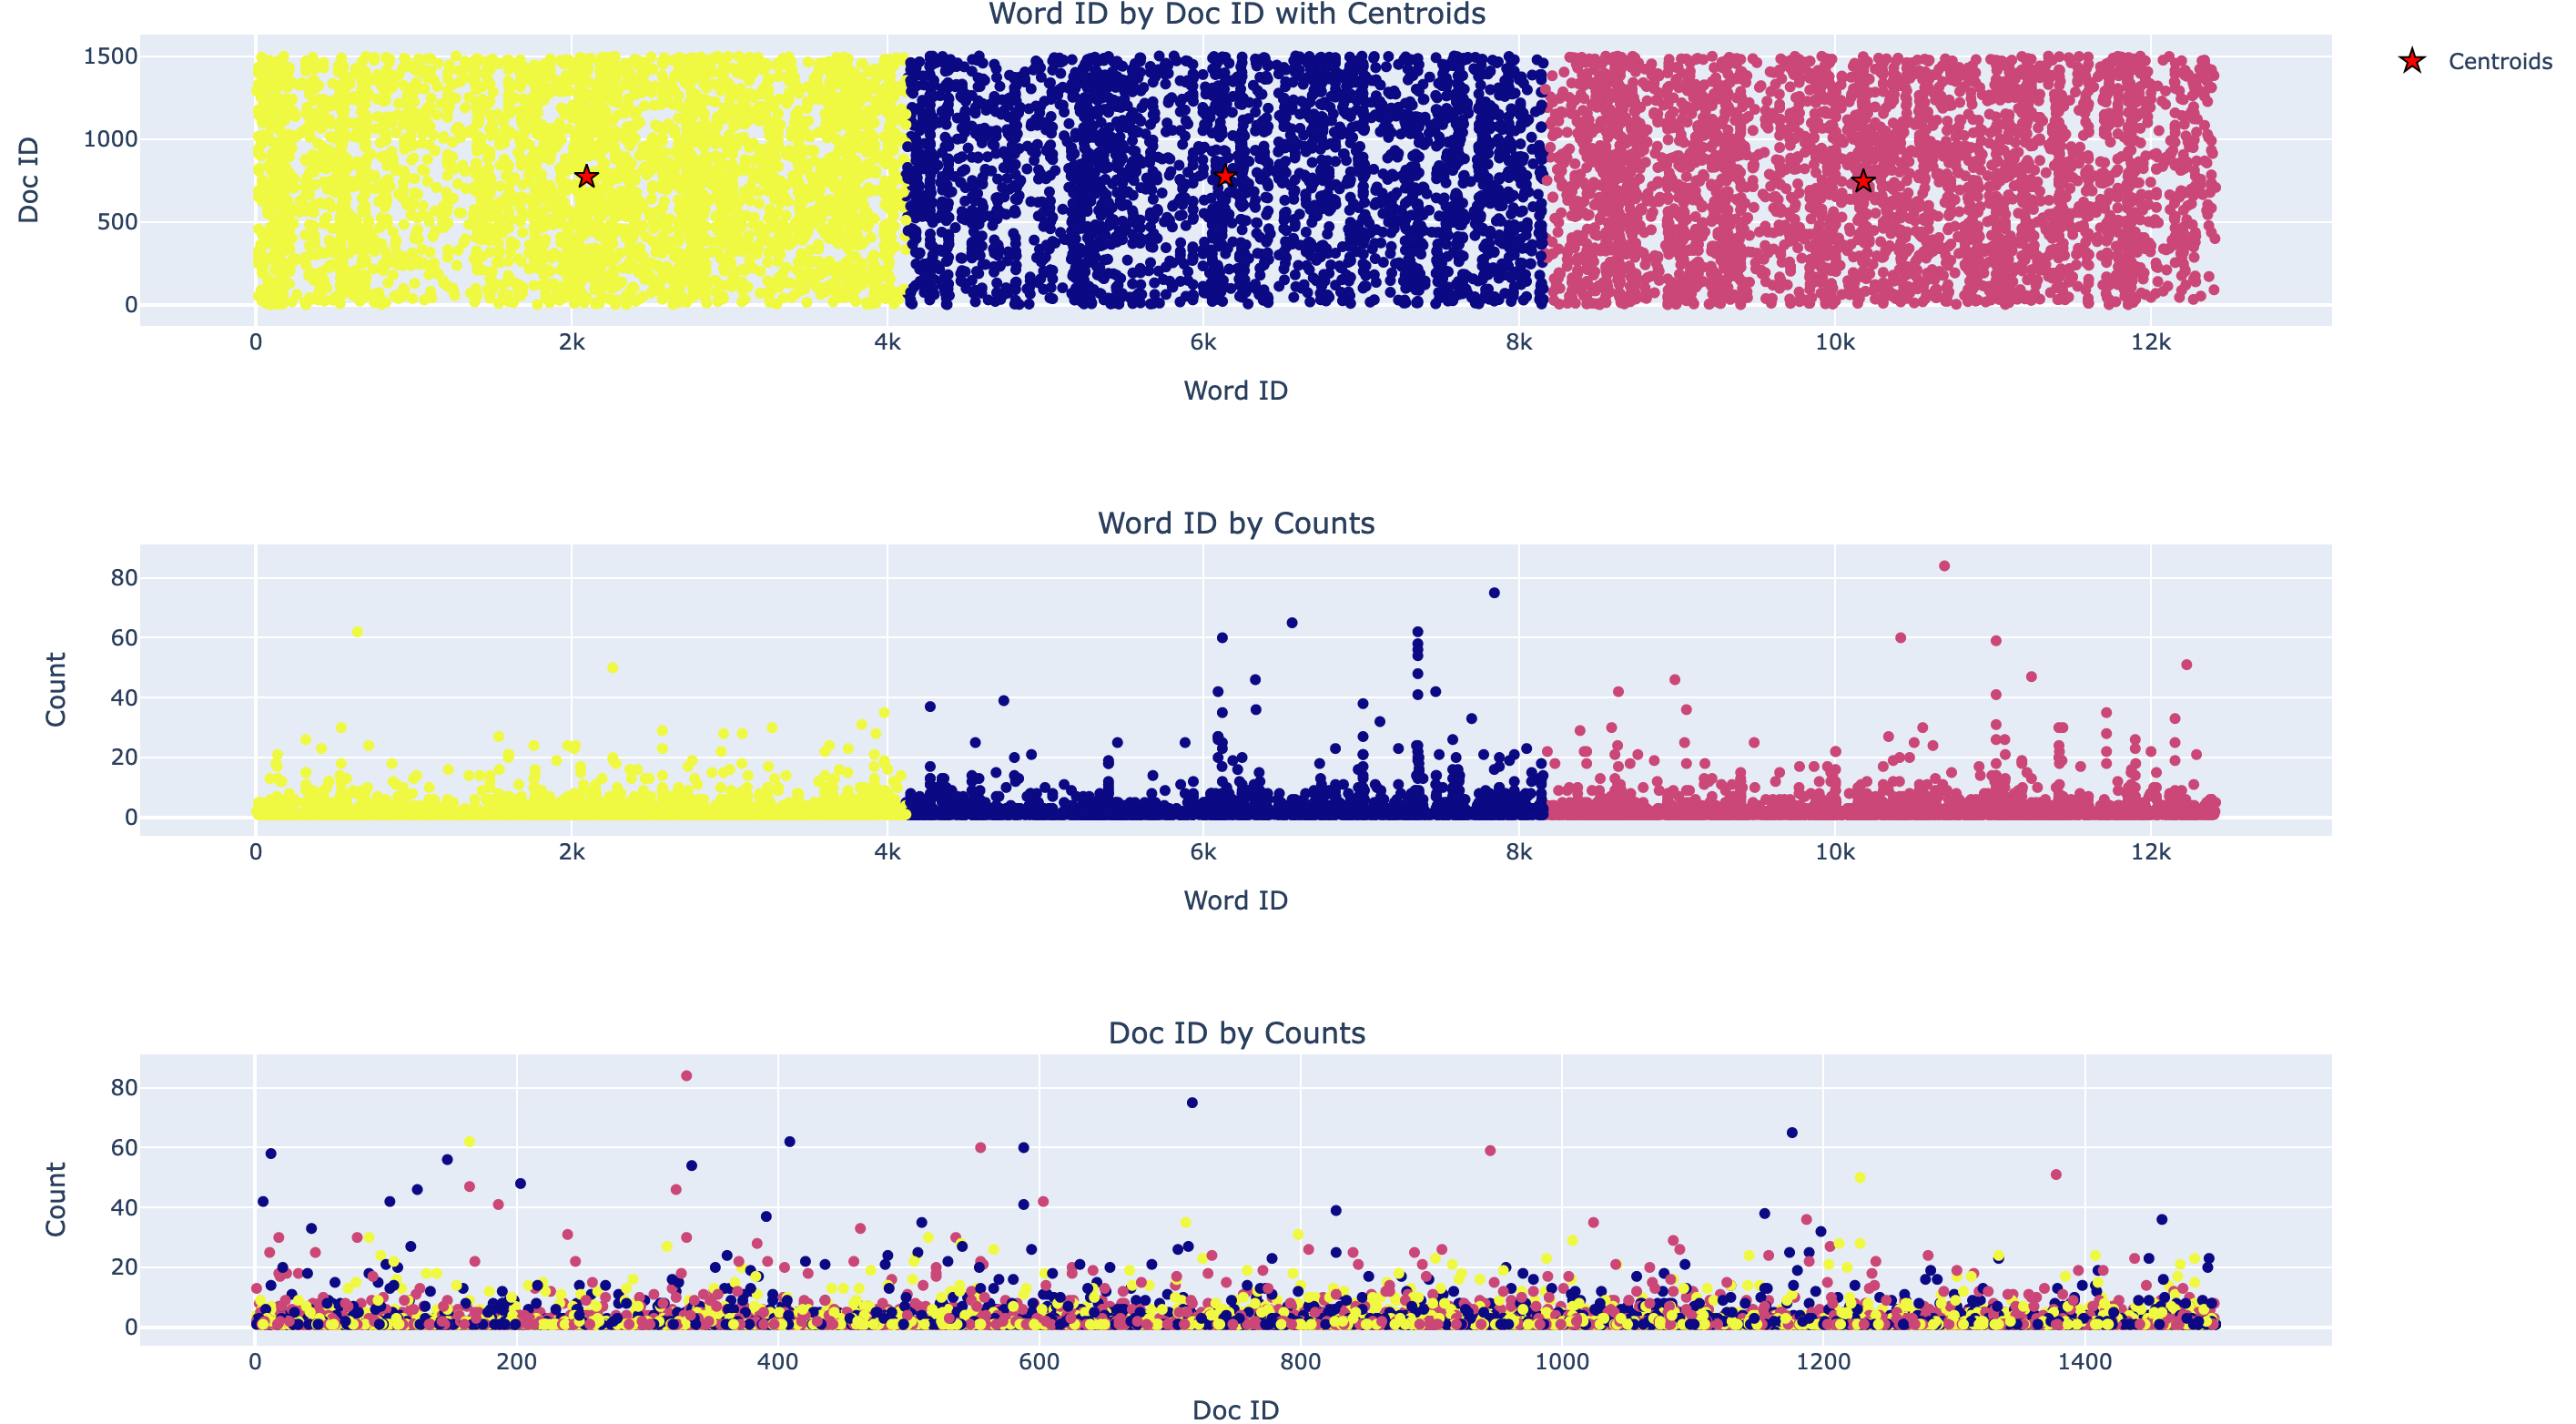
\includegraphics[width=1\textwidth]{figs/3plots.png}
\end{figure}
The first 2D plot analyzed was for the $doc\_id$ and $word\_id$ axis. It was observed that the points were evenly distributed into three clusters on the $word\_id$ axis ranging from 0 to 12419. This indicates that there were three groups of words that occurred frequently in the documents. On the other hand, the points were stacked on the $doc\_id$ axis, forming three even clusters. This suggests that there were three distinct groups of documents that contained a similar set of words. The K-means clustering algorithm identified the centroids of each of these three clusters, which were in the dead center of each cluster. This means that the algorithm correctly identified the center of each cluster and assigned the data points to the nearest centroid. However, it is important to note that this does not necessarily mean that every document in the entire dataset contains every word at least once. It only means that every document in each of these three clusters contains every word in the cluster at least once.

% In the first 2D plot analyzed for the doc_id and word_id axis, the K-means clustering algorithm identified three clusters of data points. Each cluster represents a group of documents that share a similar set of words. The fact that the points were stacked on top of each other along the word_id axis within each cluster means that every document in each of these three clusters contains every word in the cluster at least once.


% However, it is important to note that this does not necessarily mean that every document in the entire dataset contains every word at least once. It only means that every document in each of these three clusters contains every word in the cluster at least once.

The second 2D plot analyzed was for the count and $word\_id$ axis. It was observed that the points were evenly distributed into three clusters on the $word\_id$ axis ranging from 0 to 12419. This indicates that there were three groups of words that occurred frequently in the documents. However, it was also observed that the points that had counts from 1 to 10 were tightly bound together, indicating that these words occurred frequently in the documents. In contrast, the counts beyond 10 were exponentially spaced, suggesting that these words occurred less frequently in the documents.

The third 2D plot analyzed was for the count and $doc\_id$ axis. It was observed that the labeling of points of the clusters was scattered along the $doc\_id$ axis ranging from 0 to 1500. This indicates that the documents contained a diverse set of words with varying frequencies of occurrence. Additionally, it was observed that the points that had counts from 1 to 10 were tightly bound together, indicating that these documents contained a similar set of frequently occurring words. In contrast, the counts beyond 10 were exponentially spaced, suggesting that these documents contained a diverse set of less frequently occurring words
\subsection{Dimension Reduction}

In an attempt to gain more useful information from the NIPS dataset, I performed Principal Component Analysis (PCA) to reduce the dimensions of the data. PCA is a technique used to transform high-dimensional data into a lower-dimensional space while preserving the most important features of the original data\cite{medium_kmeans}. Using PCA, I reduced the three attributes ($doc\_id$, $word\_id$, count) of the NIPS dataset into two principal components: PCA 1 and PCA 2. The resulting scatter plot of the first two principal components revealed some interesting behaviors. To gain a better understanding of the data, I randomly sampled the dataset and performed the PCA analysis three times, each with a different sample size. By comparing the results of the three random samples, I was able to gain insights into the stability of the PCA analysis.

Firstly, the stacking behavior observed in the K-means clustering along the $word\_id$ axis persisted in the PCA analysis, as the clusters were still distributed along the PCA 1 axis. However, as PCA 1 increased, the spacing between points in each cluster grew greater. This suggests that the documents within each cluster became more dissimilar as PCA 1 increased.

Another behavior observed in the PCA analysis was the relationship between PCA 1 and PCA 2. As PCA 1 increased, there appeared to be a somewhat exponential increase in PCA 2, although the relationship was not strictly linear. This indicates that as the documents became more dissimilar along the PCA 1 axis, they also became more varied in terms of the word occurrences along the PCA 2 axis.



\begin{figure}[h]
    \centering
    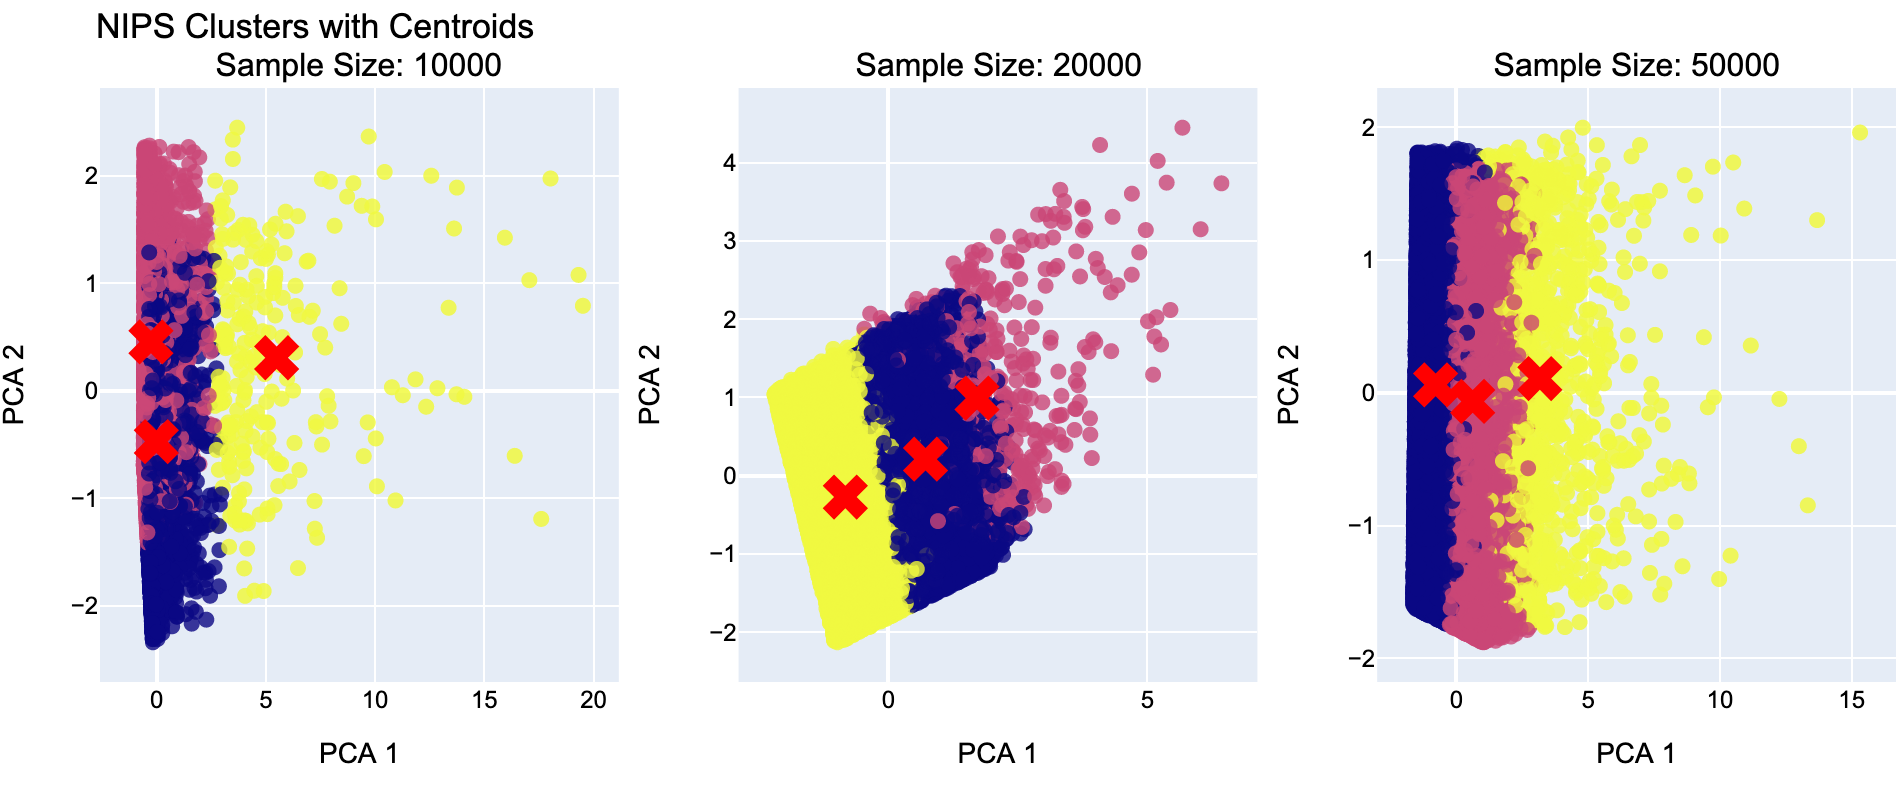
\includegraphics[width=1\textwidth]{figs/pca.png}
\end{figure}



\section{Conclusion}

The even distribution of points within each cluster on the $word\_id$ axis may be due to the nature of the dataset itself. The NIPS dataset consists of papers from various fields of research, which may share a similar vocabulary, hence the even distribution of words across the documents. Additionally, the even distribution of points on the $word_id$ axis may be a result of the K-means algorithm's assignment of data points to the nearest centroid. The algorithm tries to minimize the distance between each point and its assigned centroid, which may result in a more evenly distributed cluster.

The scattered distribution of data points along the $doc\_id$ axis in the first plot may be because the dataset has been randomly shuffled before clustering. Therefore, the data points are likely to be scattered distributed along the $doc\_id$ axis, as there is no inherent relationship or structure in the data that would cause the data points to be clustered along the $doc\_id$ axis.

The tight clustering of data points with low counts observed in both the second and third 2D plots can be attributed to the nature of the text data being analyzed. In the case of the count and $word\_id$ axis, text data typically consists of many words with very low counts and a few words with very high counts. Therefore, the tight clustering of data points with low counts in this plot suggests that there are many words with low counts in the dataset that are likely to co-occur together in documents.

Similarly, in the count and $doc\_id$ axis plot, the tight clustering of data points with low counts can be explained by the fact that many documents in the dataset contain only a few occurrences of each word. As a result, documents with low counts are more likely to occur together, while documents with high counts are more spread out across the range of $doc\_ids$. This suggests that the K-means clustering algorithm was able to identify groups of documents with similar word occurrence patterns, regardless of their position in the dataset.


In terms of our PCA analysis, the stacking behavior observed along PCA 1 axis suggests that the documents in the NIPS dataset are clustered based on the frequency of certain words. The wider spacing observed between clusters with increasing PCA 1 values may indicate that there is more variability in the word frequency patterns between clusters as the PCA 1 value increases. Additionally, the somewhat exponential increase in PCA 2 as PCA 1 increases suggests that there may be a non-linear relationship between the frequency of certain words and their co-occurrence patterns in the documents.

Overall, our analysis suggests that the K-means clustering algorithm was able to identify meaningful patterns in the NIPS dataset based on the frequency of certain words in the documents. The addition of PCA allowed us to further understand the relationship between the frequency of certain words and their co-occurrence patterns in the documents. However, the even distribution of points within each cluster on the $word\_id$ axis suggests that the dataset may have certain limitations and biases, such as a shared vocabulary among different fields of research. Nevertheless, our analysis provides valuable insights into the structure of the NIPS dataset and highlights the potential usefulness of text clustering methods in analyzing large and complex datasets.

\section{Takeaway}
Neural Information Processing Systems (NIPS) is an annual conference on machine learning and computational neuroscience. The analysis performed on NIPS papers suggests that despite the diversity of research topics presented at the conference, there may be commonalities in the language used across different fields. This could mean that researchers from different fields are able to communicate and share their ideas effectively using a shared vocabulary.

The tight clustering of data points with low counts observed in both the second and third 2D plots suggests that there are many words with low counts in the dataset that are likely to co-occur together in documents. This could mean that certain words or phrases are commonly used together across different NIPS papers, regardless of their research topic. This could facilitate cross-disciplinary communication and collaboration among researchers attending the NIPS conference.

Overall, this analysis provides some insight into the language patterns and commonalities present in NIPS papers. It could be useful for researchers looking to better understand the language used at the NIPS conference and how it relates to different research topics.


\bibliographystyle{plain}
\bibliography{ref.bib}


\end{document}
